% chapter introduction

\section{Context}

%what the subject is;
Performance monitoring of a grid is a key part in grid computing. Based on the reports of grid performance, decisions on capacity planning are being made. Visualization of performance status in different levels helps scientists and managers focus on the exact point of the infrastructure where a bottleneck on service exists.
%why you are investigating it;
Current interfaces delivers performance graphs without following the standard topology schema that is presented by the grid information system.

%which aspects you will consider, and why;
WSRF aggregation framework and GLUE schema are examined to understand the gathering process of metrics. BDII LDAP also examined as the carrier of the information data. Ganglia's hierarchical delegation to create manageable monitoring domains is an important aspect. Performance metrics are taken using Linux kernel's load average.
%which aspects you will not consider, and why;
Performance in the aspect of how many jobs are served by each site is not examined in this project.
%what you hope to find out;
This project examines which of the two information services better transfer the metrics for the multi level monitoring architecture.

%what your starting point(s) will be
A starting point was to build a lab to gather performance data and start working on the development of the integration parts.
%what assumptions you are making
It is assumed that the environment is a grid site, that already have the components needed to work together. Ganglia daemons on each node, presented by the GLUE schema on site BDII, Nagios/MyEGI monitoring frameworks.
%how you will present the subject.
A web interface is available to present the work of the integration of Ganglia into Nagios/MyEGI, BDII and WSRF.

\section{Aims \& Objectives}
%the aim and objectives of the work presented in the report

This project aims to evaluate grid performance monitoring tools, and information services to distribute that data. It will digg in depth the whole chain of data generation, distribution, provision, transformation and display using some custom built interfaces.

Using a testbed, Ganglia agent should be installed in every worker node of the Computing Element. Globus and gLite middlewares should also be installed, to provide the Information Services for data aggregation and transfer.

Resource Providers should be integrated on BDII and WSRF Information Services, to get, parse/transform and deliver the data to the front interface. Authentication mechanism is not part of this project, but in order to respect the procedures a wrapping interface such as WebMDS should be installed. Standards and specifications about data organization in the information system such as the Glue schema will be covered.

Information Services should be selected for the different levels of the Multi Level Monitoring infrastucture, such as site, regional or top level. Nagios and ganglia integration should also be evaluated.

The effect on performance by taking metrics is a problem with performance monitoring, that may be considered. Aggregation methods before display the metrics should also be used.

\section{Organization}
%TODO The dissertation should contain a section titled \sum_{anagement of Project' and the Interim Report should be bound in at the back.

\subsection[Tools]{Tools}
This project was developed in \LaTeX using Vi editor, all figures are vector graphics designed in Dia. Its releases may be found in Google Code, where Mercurial was used for source control. Citation management through Mendeley software. Papers obtained by becoming member of IEEE, ACM and USENIX. Operating Systems Laboratory of Technological Education Institute of Piraeus was used to build a testbed of grid site and tools to study existing monitoring tools.

%the initial time plan for the project work
\subsection[Time plan]{Time-plan (Gantt Chart)}

\begin{table}[ht]
\begin{tabular}{ | l | l | l | l | r |}
\hline
Task & Start date & End date & Days \\ \hline
  Preliminary & 09/29/10 & 10/24/10 & 20 \\ \hline 
  -  Identify Concepts & 09/29/10 & 10/08/10 & 8 \\ \hline 
  -  Gain Access & 10/08/10 & 10/24/10 & 12 \\ \hline 
  Planning & 11/12/10 & 12/04/10 & 17 \\ \hline 
  -  Explore existing technologies & 11/12/10 & 11/28/10 & 12 \\ \hline 
  -  Write Interim Report & 11/28/10 & 12/04/10 & 5 \\ \hline 
  Experimental-Development & 12/04/10 & 02/14/11 & 51 \\ \hline 
  -  Evaluate performance monitoring tools & 12/04/10 & 12/25/10 & 15 \\ \hline 
  -  Information Services evaluation & 12/17/10 & 12/29/10 & 8 \\ \hline 
  -  Build a testbed and test cases & 12/29/10 & 31/01/11 & 20 \\ \hline 
  -  Develop interface & 01/02/11 & 02/14/11 & 14 \\ \hline 
  Report & 02/16/11 & 03/29/11 & 32 \\ \hline 
  -  Begin Writing & 02/17/11 & 03/01/11 & 11 \\ \hline 
  -  Submit Draft \& Make Changes & 03/01/11 & 03/14/11 & 9 \\ \hline 
  -  Prepare Final & 03/14/11 & 03/29/11 & 11 \\ \hline 
\end{tabular}
\caption{Key activities necessary to complete the project}
\label{tab:tasks}
\end{table}

\tikzstyle{line} = [draw]

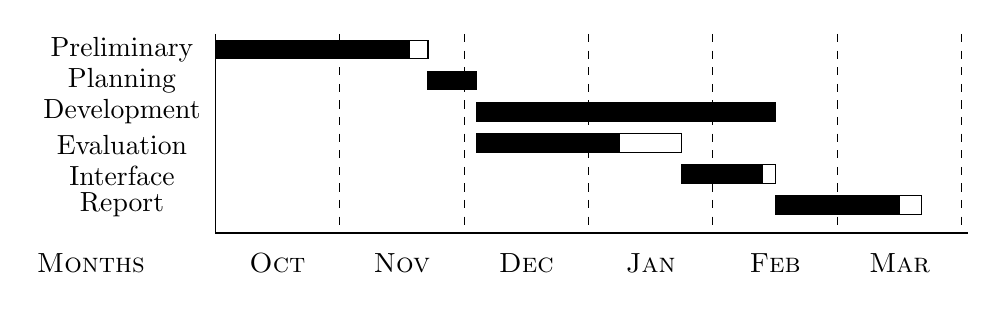
\begin{tikzpicture}[scale=0.79]
%\draw[help lines] (0,0) grid +(10,1);
%lines
\draw (0,0) -- (0,-3.2);
%\path [line,dashed] (1,0) -- (1,-5.7);
\path [line,dashed] (2,0) -- (2,-3.2);
%\path [line,dashed] (3,0) -- (3,-5.7);
\path [line,dashed] (4,0) -- (4,-3.2);
%\path [line,dashed] (5,0) -- (5,-5.7);
\path [line,dashed] (6,0) -- (6,-3.2);
%\path [line,dashed] (7,0) -- (7,-5.7);
\path [line,dashed] (8,0) -- (8,-3.2);
%\path [line,dashed] (9,0) -- (9,-5.7);
\path [line,dashed] (10,0) -- (10,-3.2);
%\path [line,dashed] (11,0) -- (11,-5.7);
\path [line,dashed] (12,0) -- (12,-3.2);

\draw (-1.5,-0.6) node[above]{Preliminary};%
\draw (-1.5,-1.1) node[above]{Planning};%
\draw (-1.5,-1.6) node[above]{Development};%
\draw (-1.5,-2.1) node[above]{Evaluation};%
\draw (-1.5,-2.6) node[above]{Interface};%
\draw (-1.5,-3.1) node[above]{Report};%
%\draw (-1.5,-3.5) node[above]{$ \textsc{activity G}$};%
%\draw (-1.5,-4) node[above]{$ \textsc{activity H}$};%
%\draw (-1.5,-4.5) node[above]{$ \textsc{activity I}$};%
%\draw (-1.5,-5) node[above]{$ \textsc{activity J}$};%
%\draw (-1.5,-5.5) node[above]{$ \textsc{Report}$};%

\filldraw[fill=white] (0,-0.1) rectangle (3.42,-0.4);% a slack
\filldraw[fill=black] (0,-0.1) rectangle (3.12,-0.4);% a
\filldraw[fill=white] (3.42,-0.6) rectangle (4.2,-0.9);% b slack
\filldraw[fill=black] (3.42,-0.6) rectangle (4.2,-0.9);% b
\filldraw[fill=black] (4.2,-1.1) rectangle (9,-1.4);% c
\filldraw[fill=white] (4.2,-1.6) rectangle (7.5,-1.9);% d slack
\filldraw[fill=black] (4.2,-1.6) rectangle (6.5,-1.9);% d
\filldraw[fill=white] (7.5,-2.1) rectangle (9,-2.4);% e slack
\filldraw[fill=black] (7.5,-2.1) rectangle (8.8,-2.4);% e
\filldraw[fill=white] (9,-2.6) rectangle (11.36,-2.9);% k slack
\filldraw[fill=black] (9,-2.6) rectangle (11,-2.9);% k
%\filldraw[fill=white] (3.2,-2.6) rectangle (6.66,-2.9);% f slack
%\filldraw[fill=black] (3.2,-2.6) rectangle (3.4,-2.9);% f
%\filldraw[fill=white] (7,-3.1) rectangle (9.6,-3.4);% g slack
%\filldraw[fill=black] (7,-3.1) rectangle (8,-3.4);% g
%\filldraw[fill=white] (7,-3.6) rectangle (7.53,-3.9);% h slack
%\filldraw[fill=black] (7,-3.6) rectangle (7.43,-3.9);% h 
%\filldraw[fill=black] (6.66,-4.1) rectangle (7.53,-4.4);% i 
%\filldraw[fill=black] (7.53,-4.6) rectangle (9.58,-4.9);% i 

\draw (0,-3.2) -- (12,-3.2);
\draw (0,-3.2) -- (12.1,-3.2);


\draw (-2,-4) node[above]{$ \textsc{Months}$};%
\draw (1,-4) node[above]{$ \textsc{Oct}$};%
%\draw (1,-6.5) node[above]{$ \textsc{21}$};%
\draw (3,-4) node[above]{$ \textsc{Nov}$};%
%\draw (3,-6.5) node[above]{$ \textsc{23}$};%
\draw (5,-4) node[above]{$ \textsc{Dec}$};%
%\draw (5,-6.5) node[above]{$ \textsc{25}$};%
\draw (7,-4) node[above]{$ \textsc{Jan}$};%
%\draw (7,-6.5) node[above]{$ \textsc{27}$};%
\draw (9,-4) node[above]{$ \textsc{Feb}$};%
%\draw (9,-6.5) node[above]{$ \textsc{29}$};%
\draw (11,-4) node[above]{$ \textsc{Mar}$};%
%\draw (11,-6.5) node[above]{$ \textsc{31}$};%
%\draw (12,-6.5) node[above]{$ \textsc{}$};%
\end{tikzpicture}




